\documentclass[greek]{beamer}
\usepackage{amsmath,amsthm} % needed for mathematics
\usepackage{unicode-math}
\usepackage{xltxtra}
\usepackage{graphicx}
\usetheme{CambridgeUS}
\usecolortheme{seagull}
\usepackage{hyperref}
\usepackage{ulem} % underline words package
\usepackage{xgreek}

\usepackage{pgfpages} 
\usepackage{tikz} % package for shapes and more
%\setbeameroption{show notes on second screen}
%\setbeameroption{show only notes}

\setsansfont{Calibri} % it is said that Calibri is the proper font for reading difficulties

\usepackage{multicol} % package for two or more columns

\usepackage{appendixnumberbeamer} % remove page numbering in appendix

\usepackage{polynom} % polynomial divisions package

\usepackage{pgffor} % macros

\setbeamercovered{highly dynamic}
\setbeamertemplate{navigation symbols}{}

\newcounter{askisi} % enviroment for exercises
\newenvironment{askisi}
{
  \refstepcounter{askisi}\par
  \subsection{Άσκηση \theaskisi}
  \begin{frame}[label=Άσκηση\theaskisi,t]{Εξάσκηση \theaskisi}
}{
  \end{frame}
}

\newcounter{lisi} % enviroment for solutions
\newenvironment{lisi}
{
  \refstepcounter{lisi}\par
  \subsection{Άσκηση \thelisi}
  \begin{frame}[label=Λύση\thelisi,t]{Λύση \thelisi}
}{
  \end{frame}
}

\title{Συναρτήσεις}
\subtitle{Θεώρημα Bolzano}
\author[Λόλας]{Κωνσταντίνος Λόλας}
\institute[$10^ο$ ΓΕΛ]{$10^ο$ ΓΕΛ Θεσσαλονίκης}
\date{}

\begin{document}

\begin{frame}
    \titlepage
\end{frame}

\section{Θεωρία}
\begin{frame}{Challenge 1}
    \begin{itemize}
        \item<1-> Φτιάξτε άξονες
        \item<2-> Σημειώστε ένα σημείο $Α$ με θετική τεταγμένη και ένα σημείο $Β$ με αρνητική
        \item<3-> Σχηματίστε συνάρτηση στο $[α,β]$ χωρίς να περάσετε από τον άξονα $x'x$
    \end{itemize}
    \onslide<4-> Συμπέρασμα...
\end{frame}

\begin{frame}{Challenge 2}
    \begin{itemize}
        \item<1-> Φτιάξτε άξονες
        \item<2-> Σημειώστε ένα σημείο $Α$ με θετική τεταγμένη και ένα σημείο $Β$ με αρνητική
        \item<3-> Σχηματίστε συνεχή συνάρτηση στο $(α,β)$ χωρίς να περάσετε από τον άξονα $x'x$
    \end{itemize}
    \onslide<4-> Συμπέρασμα...
\end{frame}

\begin{frame}{Challenge 3}
    \begin{itemize}
        \item<1-> Φτιάξτε άξονες
        \item<2-> Σημειώστε ένα σημείο $Α$ με θετική τεταγμένη και ένα σημείο $Β$ με αρνητική
        \item<3-> Σχηματίστε συνεχή συνάρτηση στο $[α,β]$ χωρίς να περάσετε από τον άξονα $x'x$
    \end{itemize}
    \onslide<4-> Συμπέρασμα...
\end{frame}

\begin{frame}{Χωρίς πολλά πολλά...}
    \begin{block}{Θεώρημα Bolzano}
        Έστω μια συνάρτηση $f$ ορισμένη σε κλειστό διάστημα $[α,β]$. Αν:
        \begin{itemize}
            \item η $f$ είναι συνεχής στο $[α,β]$ και
            \item $f(α)\cdot f(β)<0$,
        \end{itemize}
        τότε υπάρχει $x_0\in (α,β)$ τέτοιο ώστε $f(x_0)=0$
    \end{block}
\end{frame}

\begin{frame}{Παρατηρήσεις}
    \begin{itemize}
        \item<1-> ΔΕΝ είναι τρόπος επίλυσης εξισώσεων
        \item<2-> ΔΕΝ βρίσκει - εντοπίζει ρίζες
        \item<3-> ΔΕΝ τις μετράει σε πλήθος
    \end{itemize}
    \onslide<4->Το μόνο που κάνει είναι να σε πληροφορεί ότι ΣΙΓΟΥΡΑ έχει ρίζα μια συνάρτηση. \onslide<5-> ΜΟΝΟ
\end{frame}

\begin{frame}{Τεστ μνήμης - ικανοτήτων}
    Πώς επιλύουμε εξισώσεις αλγεβρικά?
    \begin{itemize}
        \item<1-> Προφανής ρίζα
        \item<2-> Λύνουμε ως προς $x$
        \item<3-> Παραγοντοποίηση
        \item<4-> 1-1
    \end{itemize}
\end{frame}

\begin{frame}[noframenumbering]
    Στο moodle θα βρείτε τις ασκήσεις που πρέπει να κάνετε, όπως και αυτή τη παρουσίαση
\end{frame}

\section{Ασκήσεις}

\begin{frame}[noframenumbering]
    \vfill
    \centering
    \begin{beamercolorbox}[sep=8pt,center,shadow=true,rounded=true]{title}
        \usebeamerfont{title}Ασκήσεις
    \end{beamercolorbox}
    \vfill
\end{frame}

\begin{askisi}
    Να αποδείξετε ότι:
    \begin{enumerate}
        \item<1-> Η συνάρτηση $f(x)=x^3+x-1$ ικανοποιεί τις υποθέσεις του θεωρήματος Bolzano στο διάστημα $[0,1]$.
        \item<2-> Η εξίσωση $x^3+x-1=0$ έχει μία τουλάχιστον ρίζα στο διάστημα $(0,1)$.
    \end{enumerate}

    %\hyperlink{Λύση1}{\beamerbutton{Λύση}}
\end{askisi}

\begin{askisi}
    Να αποδείξετε ότι υπάρχει ένα τουλάχιστον $x_0\in (0,1)$ τέτοιο ώστε $x_0^2+3x_0=e^{x_0}+1$.

    %\hyperlink{Λύση2}{\beamerbutton{Λύση}}
\end{askisi}

\begin{askisi}
    Έστω $f:\mathbb{R}\to\mathbb{R}$ μία συνάρτηση η οποία είναι συνεχής με $f(\mathbb{R})=(0,1)$. Να αποδείξετε ότι η εξίσωση $f(x)=x-1$ έχει μία τουλάχιστον ρίζα στο διάστημα $(1,2)$.

    %\hyperlink{Λύση3}{\beamerbutton{Λύση}}
\end{askisi}

\begin{askisi}
    Να αποδείξετε ότι η εξίσωση $\dfrac{e^x}{x-2}+\dfrac{x^2+1}{x-1}=0$ έχει μία τουλάχιστον ρίζα στο διάστημα $(1,2)$.

    %\hyperlink{Λύση4}{\beamerbutton{Λύση}}
\end{askisi}

\begin{askisi}
    Να αποδείξετε ότι υπάρχει μοναδικό $x_0\in (0,1)$ τέτοιο ώστε $e^{x_0}+x_0=2$

    %\hyperlink{Λύση5}{\beamerbutton{Λύση}}
\end{askisi}

\begin{askisi}
    Δίνονται οι συναρτήσεις $f(x)=\ln x$ και $g(x)=\dfrac{1}{x}$. Να αποδείξετε ότι οι $C_f$ και $C_g$ στο διάστημα $(1,e)$ έχουν ένα ακριβώς κοινό σημείο.

    %\hyperlink{Λύση6}{\beamerbutton{Λύση}}
\end{askisi}

\begin{askisi}
    Να αποδείξετε ότι η εξίσωση $x^3-4x^2+2=0$ έχει δύο τουλάχιστον ρίζες στο διάστημα $(-1,1)$.

    %\hyperlink{Λύση7}{\beamerbutton{Λύση}}
\end{askisi}

\begin{askisi}
    Δίνεται το ορθογώνιο $ΟΑΒΓ$ του σχήματος και μία συνεχής συνάρτηση $f$ στο $[0,2]$ της οποίας η γραφική παράσταση βρίσκεται στο χωρίο που ορίζει το ορθογώνιο. Να αποδείξετε ότι η $C_f$ τέμνει τη διαγώνιο $ΑΓ$.

    \centering
    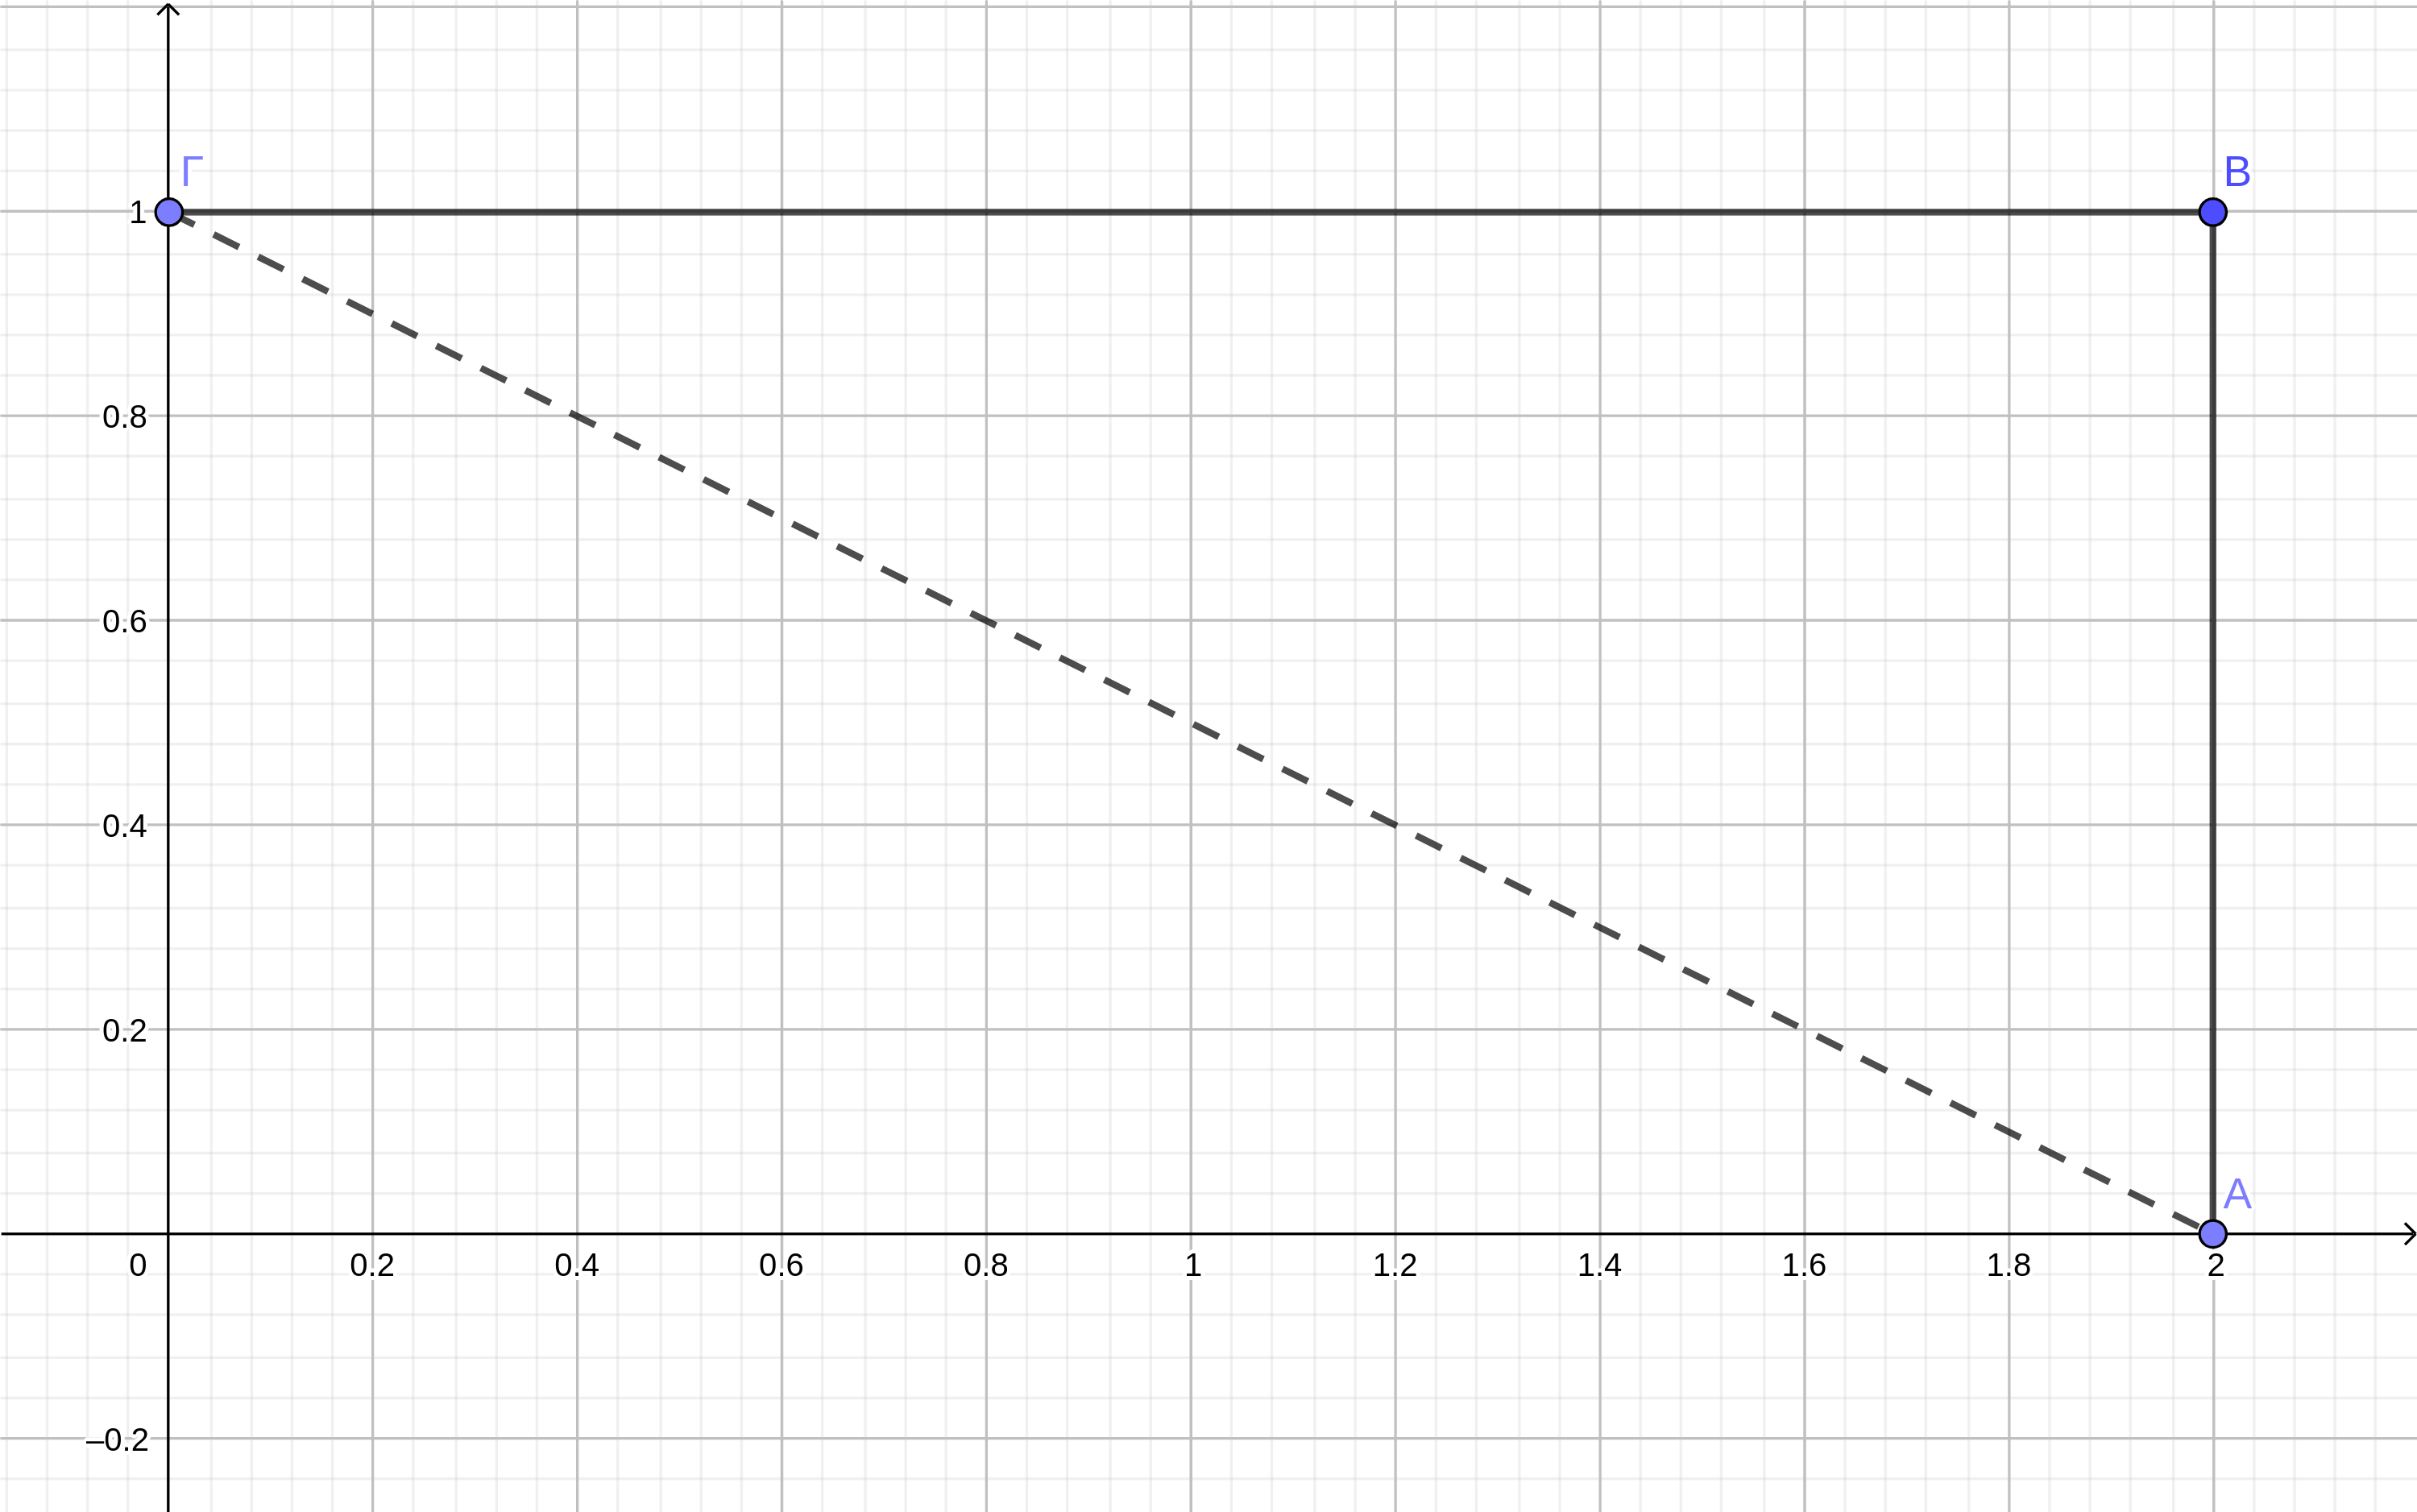
\includegraphics[width=0.5\textwidth]{"images/Bolzano.png"}

    %\hyperlink{Λύση8}{\beamerbutton{Λύση}}
\end{askisi}

\begin{askisi}
    Να δείξετε ότι η εξίσωση $\ln x=\dfrac{1}{x-1}$ έχει μία τουλάχιστον ρίζα στο διάστημα $(0,1)$.

    %\hyperlink{Λύση9}{\beamerbutton{Λύση}}
\end{askisi}

\begin{askisi}
    Έστω η συνεχής συνάρτηση $f:[0,1]\to\mathbb{R}$ με $-1<f(x)<0$, για κάθε $x\in [0,1]$. Να δείξετε ότι υπάρχει ένα τουλάχιστον $x_0\in (0,1)$ τέτοιο ώστε $f^2(x_0)=2f(x_0)+3x_0$

    %\hyperlink{Λύση10}{\beamerbutton{Λύση}}
\end{askisi}

\end{document}
